\documentclass[11pt]{article}

\usepackage{graphicx,amsmath,amssymb,subfigure,url,xspace,textcomp,booktabs,siunitx,
  todonotes}
\usepackage{todonotes}
\usepackage[utf8]{inputenc}
\usepackage[bf]{caption}
\usepackage[
backend=bibtex,
style=numeric,
sortlocale=de_DE,
natbib=true,
url=false, 
doi=true,
eprint=false
]{biblatex}

\addbibresource{../sources.bib}

\newcommand{\eg}{e.g.,\xspace}
\newcommand{\bigeg}{E.g.,\xspace}
\newcommand{\etal}{\textit{et~al.\xspace}}
\newcommand{\etc}{etc.\@\xspace}
\newcommand{\ie}{i.e.,\xspace}
\newcommand{\bigie}{I.e.,\xspace}


\title{Measurement of electrical properties (current-voltage and capacitance-voltage) of irradiated and non-irradiated silicon detectors}
\author{Michael Larson, Elisabeth Unger, Samuel Flis, Christian Bourjau}

\begin{document}
\maketitle
\begin{itemize}
\item Give a brief description of the setup and measurements.
\item Plot capacitance and leakage current in function of applied bias voltage for all samples.
\item Determine depletion voltage for all samples.
\item Compare the leakage current at a fixed voltage (e.g. 50 V) for all samples in one plot.
\item Describe the changes in behaviour of the irradiated detector.
\item Why it is important to measure leakage current?
\item What kind of information about the detector can be obtained from the CV data? From IV data?
\item Which polarity of bias voltage do you apply and why?
\end{itemize}

\section{Introduction}
\label{sec:introduction}

Semiconductor sensors are omnipresent in the field of particle physics.
They are also deployed in areas exhibiting a large dose of radiation like the inner tracking system of collider based experiments.
Therefore, it is crucial to understand the electrical properties and the response to radiation of these kind of detectors.
This laboratory exercise explores the  properties of Si based sensors by measuring the current and capacity of these devices as a function of the applied reverse bias $V$.
These measurements allow us to determine the depletion voltage of the given samples as well as to qualitatively observe the effect of radiation.

Applying and increasing a $V$ to a diode will lead to a growing depletion region until the entire volume of a pn-junction is free of free charge carriers.
At this point, $V_{fd}$, the diode is said to be fully depleted.
The depleted volume is free of charge carriers and hence acts as an insulator in an electric field. $V_{fd}$ depends on the geometry and material of the diode.
Assuming a flat pn-junction, $V_{fd}$ is given by
\begin{equation}
  \label{Vfd}
  V_{fd} = \frac{qN_{eff}d^2}{2\epsilon_0\epsilon_r}
\end{equation}
where $q$ is the elementary charge ($\SI{1.6e-19}{C}$), $N_{eff}$ is the effective charge density at the boundary of the deleted region, $d$ is the length of the depleted region and $\epsilon_0 = \SI{8.85e-12}{F/m}$ is the vacuum permittivity and $\epsilon_r$ is the permittivity of the material in the depleted region ($\epsilon_r^{Si} = 11.68$)\todo{add source}.
The depleted region represents the active volume used for detection and its size $d$ can be deduced by rearranging\eqref{Vfd}. 
Furthermore, the presence of two oppositely charged surfaces separated by an insulator provides the geometry of a parallel plate capacitor. Thus, the capacity of the depleted diode can be expressed, using \eqref{Vfd}, as
\begin{equation}
  \label{C}
  C = \frac{\epsilon_{0}\epsilon_{r}A}{d}
\end{equation}
where $A$ is the area of one of the boundaries of the depleted region. Since the capacity is governed by $d$ it will only increase with the applied $V$ until the diode is fully depleted. For $V \geq V_{fd}$, the capacity of the diode is given by
\begin{equation}
  \label{eq:1}
   C_{fd} = A \sqrt{\frac{\epsilon_0\epsilon_rqN_{eff}}{2V}}
\end{equation}
However, due to thermal excitations within the depleted region, a leakage current is present whenever a voltage is applied to the diode.
At full depletion, the leakage current only depends on the rate at which electron-hole pairs are generated. Thus, $I(V)$ exhibits a plateau for $V>V_{fd}$.

\section{Samples and measurement}
\label{sec:samples}
During this exercise, the current-voltage and capacity-voltage relation of three different diodes were studied. While all samples were Si based, they differed in the type of doping used in their bulk region and in their exposure to radiation.
Presented here are the measurements of a non-irradiated p-type diode, a non-irradiated n-type diode and a second n-type diode irradiated by syncrotron radiation. 

The measurements were conducted in a clean room environment. 
Connection to the anode and cathode of each diode were achieved by placing a probe needle onto the sample.
The polarity of the applied voltage was selected to be opposite that of the diode, causing the creation of a depletion region.
Furthermore, the experiment was shielded from light to avoid charge buildup due to the photoelectric effect. Subsequently, the current and capacity of the diodes were measured over a range of different voltages. Each measurement was repeated 3 times in order to minimize statistical fluctuations and to investigate the systematic error of the experimental setup.

The diodes were scanned over a limited voltage range in order to avoid creating an avalanche discharge due to a thermal electron-hole pairs.

\section{Results}
Fig.~\ref{fig:cv} displays the diodes' inverse squared capacitance, $\frac{1}{C^{-2}}$ and the applied voltage $V$.
A plateau of $1/C^2$ can be observed for all three diodes.
However, large deviations between the successive measurements was observed for the p-typed diode. These might have been caused by residual charges slowly draining in between successive measurements.
Discussions with more experienced collegues indicated that the equipment has known inaccuracies when measuring small capacitances of order of $\sim pF$. The absolute scale of the capacitance therefore cannot be relied upon, but the shape is reproducible between different measurements.
$V_{fd}$ is estimated by fitting linear functions to the rising and plateaued regions. 

\begin{table}[]
\centering
\begin{tabular}{lllll}
                               & \multicolumn{2}{l}{Undepleted Region}                                                                                               & \multicolumn{2}{l}{Depleted Region}                                                                                                \\
                               & Slope ($10^{-6}pF^{-2}V^{-1}$)) & Intercept ($10^{-3}pF^{-2}$) & Slope ($10^{-6}pF^{-2}V^{-1}$) & Intercept ($10^{-3}pF^{-2}$) \\
Sample 8, P-Type               & 7.7\pm4.6                                                                 & 37.3\pm0.8                                              & 441.9\pm23.5                                                             & 5.0\pm0.3                                               \\
Sample 12, N-Type              & 22.6\pm4.9                                                                & 7.3\pm0.4                                               & 171.7\pm2.7                                                              & -2.1\pm0.1                                              \\
Sample 18, N-Type (Irradiated) & 12.4\pm37.5                                                               & 58.0\pm3.0                                              & 1978.6\pm110.3                                                           &                                                        
\end{tabular}
\end{table}

 The intersection of the two functions is defined as $V_{fd}$.
Under this definition, it becomes clear that the radiation damage of the n-doped diode causes an increase in $V_{fd}$: from \SI{25.16\pm0.20}{V} (not irradiated) to \SI{63.04\pm2.90}{V} (irradiated).
\label{sec:results}
\begin{figure}
  \centering
  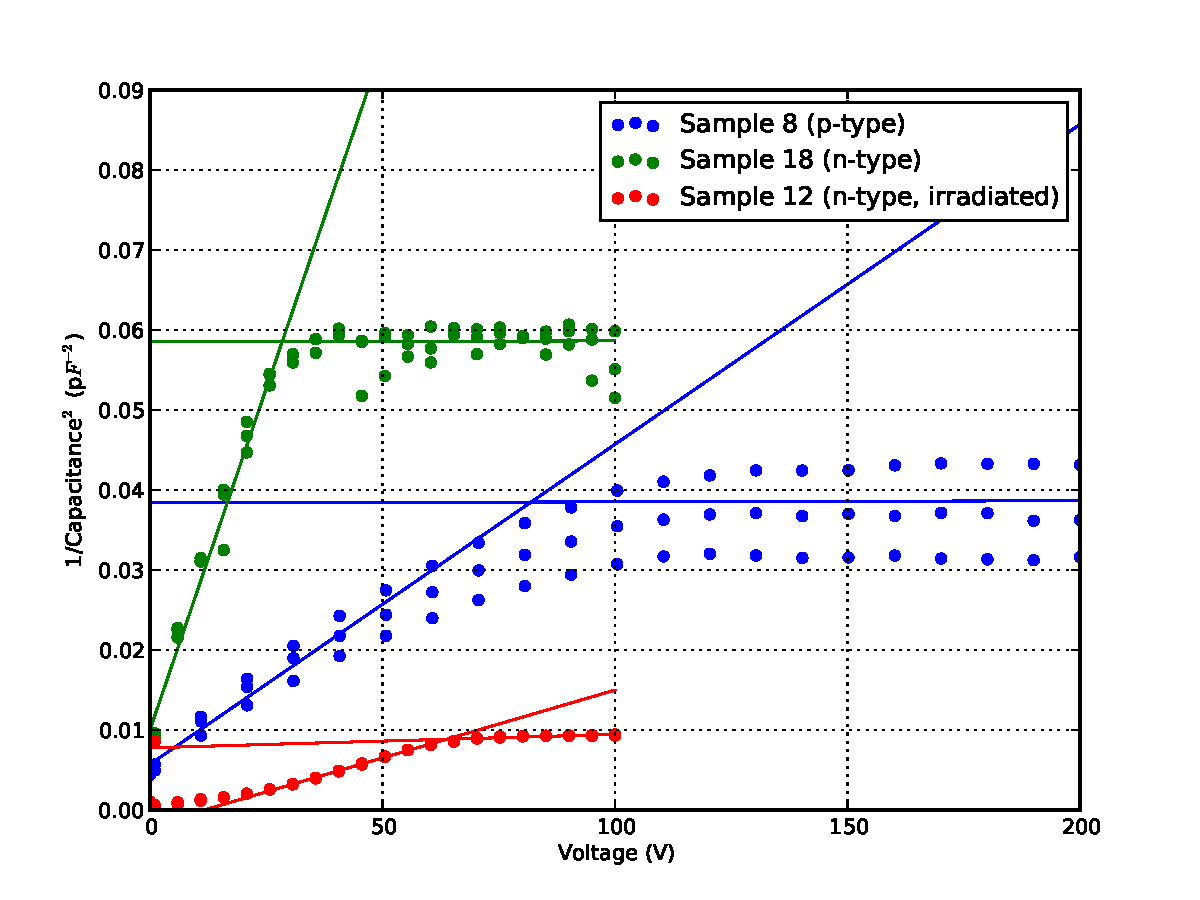
\includegraphics[width=\textwidth]{./figures/cv.pdf}  
  \caption{Capacity-Voltage }
  \label{fig:cv}
\end{figure}

Fig.~\ref{fig:iv} displays the diodes' $I$-$V$ curves whereas the shaded area represent the spread observed in the three measurements.
The voltage ranges are identical with the ones used in the $C-V$ measurement.
The flattening of $I$ for $V>V_{fd}$ can clearly be seen in the n-doped samples.
Furthermore, the effect of the radiation damage is striking.
The leakage current increased by $\sim 3$ orders of magnitude compared to the non-irradiated n-typed diode.

\begin{figure}
  \centering
  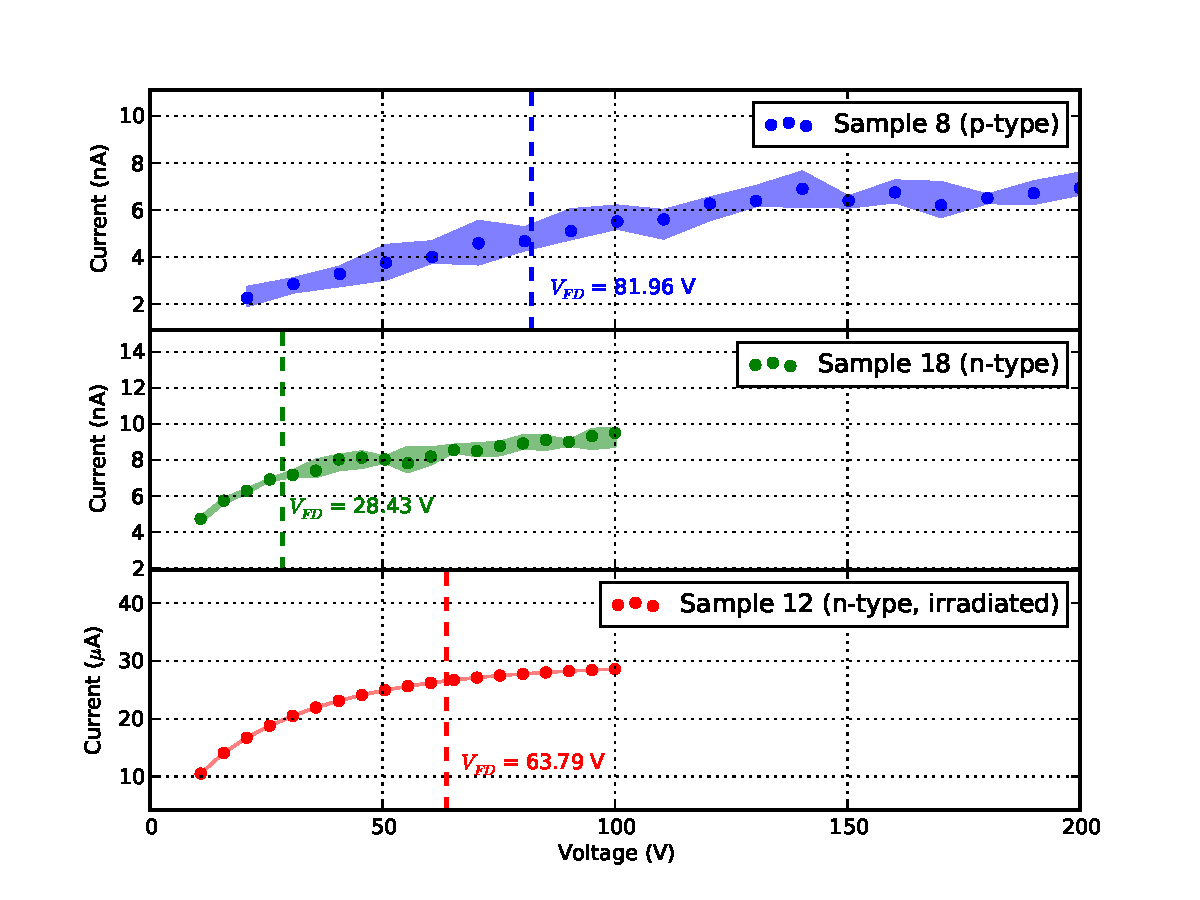
\includegraphics[width=\textwidth]{./figures/iv.pdf}
  \caption{Current-voltage}
  \label{fig:iv}
\end{figure}

\section{Summary}
\label{sec:summary}
The $C-V$ and $I-V$ curves of three different diodes were successfully measured.
While the scale of $C$ was found to not be reliable, their shapes were reproducible in repeated measurements.
Based on these shapes it was possible to determine $V_{fd}$ for each diode and to observe the plateau in both curves for $V>V_{fd}$.
Radiation damage was found to cause an increase in $V_{fd}$ by a factor of $\sim 3$ and $I$ by a three orders of magnitude.
This significant increase of the leakage current causes a deterioration of the signal-to-noise ratio in particle detectors.

\printbibliography

\end{document}

%%% Local Variables:
%%% mode: latex
%%% TeX-master: t
%%% End:
